\documentclass[11pt]{article}
\usepackage[utf8]{inputenc}
\usepackage[T1]{fontenc}
\usepackage{amsmath}
\usepackage{amssymb} % Needed for \eth
\usepackage{graphicx}
\usepackage{geometry}
\usepackage{tikz}
\usepackage{pgfplots} % For plots
\usepackage{ulem}     % For underline, using normalem to avoid messing with \emph
\usetikzlibrary{calc}
\geometry{a4paper, margin=1in}
\usetikzlibrary{positioning, arrows.meta, shapes.geometric, patterns} % For TikZ diagrams
\pgfplotsset{compat=1.18} % Use a recent PGFPlots version

% Custom commands (optional)
\newcommand{\avg}[1]{\overline{#1}}
\newcommand{\prob}[1]{P(#1)}
\newcommand{\ProbDens}[1]{\mathcal{P}(#1)} % Using script P for density
\newcommand{\vect}[1]{\vec{#1}}
\newcommand{\dd}[1]{\mathrm{d}#1} % Differential d
\newcommand{\pderiv}[2]{\frac{\partial #1}{\partial #2}}
\newcommand{\deriv}[2]{\frac{\mathrm{d} #1}{\mathrm{d} #2}}
\newcommand{\muState}{\mu\text{-state}} % Microstate
\newcommand{\OmegaE}{\Omega(E)}
\newcommand{\omegaE}{\omega(E)}
\newcommand{\PhiE}{\Phi(E)}
\newcommand{\deltaE}{\delta E}
\newcommand{\ethbar}{\text{\it{đ}}} % \eth symbol for inexact differential
\newcommand{\kb}{k_B} % Boltzmann constant
\newcommand{\gasR}{R} % Ideal gas constant

\title{Physics 415 - Lecture 16: Heat Engines and Refrigerators}
\date{February 26, 2025}
\author{} % Author not specified

\begin{document}

\maketitle
\thispagestyle{empty}

\section*{Summary}

\begin{itemize}
    \item First Law: $\Delta E = Q - W$. ($Q$=heat absorbed by system, $W$=work done by system). Differential form: $dE = \ethbar Q - \ethbar W$.
    \item Second Law: For an isolated system, total entropy change $\Delta S_{tot} \ge 0$.
        \begin{itemize}
            \item $\Delta S_{tot} > 0$: Irreversible process.
            \item $\Delta S_{tot} = 0$: Reversible process.
        \end{itemize}
    \item Heat Bath/Reservoir: A very large system at temperature $T$. If it absorbs heat $Q$ reversibly, its entropy changes by $\Delta S = Q/T$. Its temperature change $\Delta T = Q/C$ is negligible (assumed $C \to \infty$).
\end{itemize}

\section*{Heat Engines \& Refrigerators}

\subsection*{Heat Engine}
A device (thermodynamic system) that operates in a cycle, absorbs heat, and converts part of this energy to work.
In more detail:
\begin{itemize}
    \item Device M (working substance) undergoes a cyclic process.
    \item In each cycle:
        \begin{itemize}
            \item Heat $q_1$ is absorbed from a high-temperature reservoir ($T_1$).
            \item Part of this energy is converted to work $W$.
            \item Remaining heat $q_2$ is dumped to a lower-temperature reservoir ("heat sink") ($T_2 < T_1$).
        \end{itemize}
\end{itemize}
The laws of thermodynamics ultimately limit the efficiency of such a heat engine.

\textbf{A "Perfect" Heat Engine?}
Could an engine, in each cycle, convert *all* absorbed heat $q_1$ into work $W=q_1$, with $q_2=0$?

\begin{center}
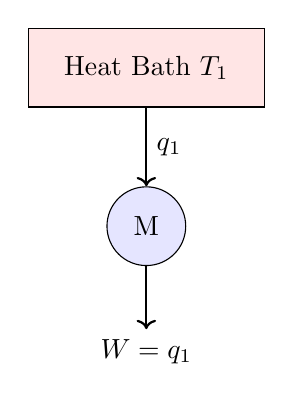
\begin{tikzpicture}
    \node (Bath) [draw, fill=red!10, minimum width=3cm, minimum height=1cm, label=center:Heat Bath $T_1$] {};
    \node (M) [draw, circle, fill=blue!10, minimum size=1cm, below=1cm of Bath, label=center:M] {};
    \draw [->, thick] (Bath.south) -- (M.north) node[midway, right] {$q_1$};
    \draw [->, thick] (M.south) -- ++(0,-0.8) node[below] {$W=q_1$};
\end{tikzpicture}
\end{center}

Such a device would not violate the First Law ($\Delta E_M = 0$ over cycle, $Q_{net} = q_1$, $W = q_1 \implies \Delta E_M = Q_{net} - W = 0$).
However, the Second Law forbids such a machine. Let's analyze the total entropy change over one cycle:
\[ \Delta S_{tot} = \Delta S_{M} + \Delta S_{heat\_bath} \]
Since M returns to its initial state after a cycle, $\Delta S_M = 0$.
The heat bath loses heat $q_1$, so its entropy change is $\Delta S_{heat\_bath} = -q_1 / T_1$.
\[ \implies \Delta S_{tot} = 0 + (-\frac{q_1}{T_1}) = -\frac{q_1}{T_1} \]
If the engine does positive work, $W=q_1>0$. Then $\Delta S_{tot} = -W/T_1 < 0$.
This contradicts the Second Law ($\Delta S_{tot} \ge 0$). X
(If $W \le 0$, the process is allowed but useless as an engine).

\textbf{Kelvin's Statement of the Second Law:} "It is impossible to construct a perfect heat engine" (a device whose sole effect is to extract heat from a reservoir and convert it entirely into work).

From a statistical viewpoint: A perfect heat engine would require the spontaneous occurrence of a process in which some amount of energy, distributed randomly among the enormous number of degrees of freedom (DOF) of the bath, converts entirely into the ordered motion of a single DOF doing work (e.g., piston). This would correspond to a decrease in total entropy $S$, which is overwhelmingly improbable.

\textbf{A "Real" Heat Engine (with two reservoirs):}
By introducing another heat bath at lower temperature $T_2$, where entropy increases, we can satisfy the Second Law:

\begin{center}
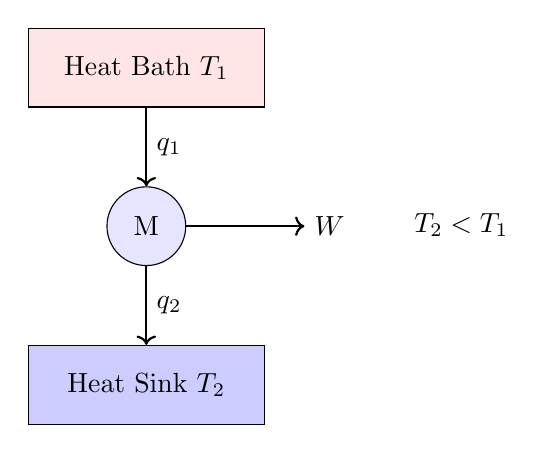
\begin{tikzpicture}
    \node (Bath1) [draw, fill=red!10, minimum width=3cm, minimum height=1cm, label=center:Heat Bath $T_1$] {};
    \node (M) [draw, circle, fill=blue!10, minimum size=1cm, below=1cm of Bath1, label=center:M] {};
    \node (Bath2) [draw, fill=blue!20, minimum width=3cm, minimum height=1cm, below=1cm of M, label=center:Heat Sink $T_2$] {};
    \draw [->, thick] (Bath1.south) -- (M.north) node[midway, right] {$q_1$};
    \draw [->, thick] (M.east) -- ++(1.5, 0) node[right] {$W$};
    \draw [->, thick] (M.south) -- (Bath2.north) node[midway, right] {$q_2$};
    \node at (4, -2) {$T_2 < T_1$};
\end{tikzpicture}
\end{center}

Assume a cyclic process for M ($\Delta S_M = 0$).
First Law: $\Delta E_M = (q_1 - q_2) - W = 0 \implies W = q_1 - q_2$. ($q_1, q_2, W$ are all positive quantities here).
Second Law: $\Delta S_{tot} = \Delta S_1 + \Delta S_2 + \Delta S_M \ge 0$.
$\Delta S_1 = -q_1/T_1$ (heat leaves reservoir 1).
$\Delta S_2 = +q_2/T_2$ (heat enters reservoir 2).
\[ \Delta S_{tot} = -\frac{q_1}{T_1} + \frac{q_2}{T_2} \ge 0 \]
Substitute $q_2 = q_1 - W$:
\[ -\frac{q_1}{T_1} + \frac{q_1 - W}{T_2} \ge 0 \]
\[ \frac{q_1}{T_2} - \frac{W}{T_2} \ge \frac{q_1}{T_1} \]
\[ \frac{W}{T_2} \le q_1 \left( \frac{1}{T_2} - \frac{1}{T_1} \right) = q_1 \frac{T_1 - T_2}{T_1 T_2} \]
\[ W \le q_1 \frac{T_1 - T_2}{T_1} = q_1 \left( 1 - \frac{T_2}{T_1} \right) \]
This inequality limits the maximum work obtainable from heat $q_1$.

Define the "efficiency" $\eta$ of the engine:
\[ \eta = \frac{W}{q_1} = \frac{\text{what we get out (Work)}}{\text{what we put in (Heat } q_1 \text{)}} \]
The Second Law implies:
\[ \eta \le 1 - \frac{T_2}{T_1} \]
An efficient engine requires $T_2 \ll T_1$ (large temperature difference: high $T_1$, low $T_2$).

The maximum possible efficiency is achieved for a reversible process, where $\Delta S_{tot} = 0$.
\[ \eta_{max} = 1 - \frac{T_2}{T_1} = \frac{T_1 - T_2}{T_1} \]
This maximum efficiency is called the \textbf{Carnot Efficiency}.
Roughly, a reversible engine avoids "friction" and processes that generate entropy, like heat transfer across large temperature differences.

\subsection*{Carnot Cycle}
An example of a reversible cycle that achieves the maximum efficiency is the Carnot cycle. It consists of four reversible steps carried out on a working substance (e.g., gas, liquid):

\begin{enumerate}
    \item[(a)] Isothermal expansion at $T=T_1$. Heat $q_1$ absorbed from reservoir 1.
    \item[(b)] Adiabatic expansion ($Q=0$). Temperature drops from $T_1$ to $T_2$.
    \item[(c)] Isothermal compression at $T=T_2$. Heat $q_2$ given off to reservoir 2.
    \item[(d)] Adiabatic compression ($Q=0$). Temperature rises from $T_2$ to $T_1$.
\end{enumerate}

\begin{center}
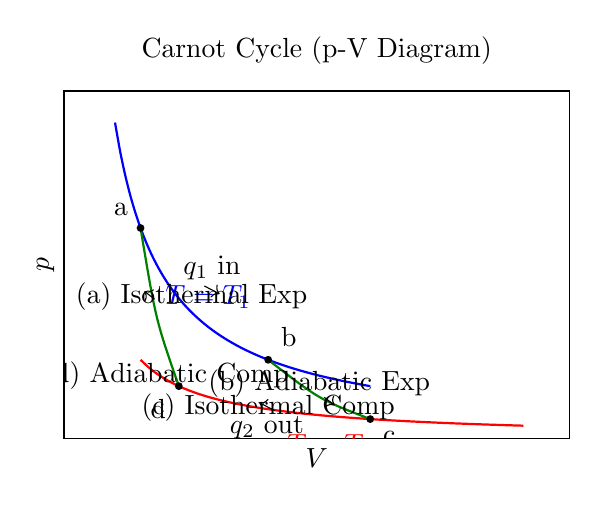
\begin{tikzpicture}
\begin{axis}[
    xlabel=$V$, ylabel=$p$,
    xmin=0, ymin=0,
    xtick=\empty, ytick=\empty,
    width=8cm, height=6cm,
    title={Carnot Cycle (p-V Diagram)}
]
% Isotherms
\addplot [domain=1:6, samples=50, smooth, thick, blue] {4/x} node[pos=0.5, anchor=south, yshift=3pt] {$T=T_1$};
\addplot [domain=1.5:9, samples=50, smooth, thick, red] {1.5/x} node[pos=0.5, anchor=north, yshift=-3pt] {$T=T_2$};
% Adiabats (steeper than isotherms)
\coordinate (a) at (axis cs:1.5, {4/1.5});
\coordinate (b) at (axis cs:4, {4/4});
\coordinate (c) at (axis cs:6, {1.5/6}); % Vc needed to connect via adiabat
\coordinate (d) at (axis cs:2.25, {1.5/2.25}); % Vd needed to connect via adiabat

% Manually define adiabatic curves (schematic, make steeper)
\draw[thick, green!50!black] (b) .. controls (5, 0.5) .. (c);
\draw[thick, green!50!black] (d) .. controls (1.8, 1.5) .. (a);

% Labels and Arrows
\node at (a) [circle, fill=black, inner sep=1pt, label=above left:a] {};
\node at (b) [circle, fill=black, inner sep=1pt, label=above right:b] {};
\node at (c) [circle, fill=black, inner sep=1pt, label=below right:c] {};
\node at (d) [circle, fill=black, inner sep=1pt, label=below left:d] {};

\draw [->] ($(a)!0.5!(b)$) + (0,0.1) -- +(0.3, 0) node[midway, above] {$q_1$ in}; % a->b
\draw [->] ($(b)!0.5!(c)$) + (0.1,-0.1) -- +(0.3, -0.2); % b->c
\draw [->] ($(c)!0.5!(d)$) + (0,-0.1) -- +(-0.3, 0) node[midway, below] {$q_2$ out}; % c->d
\draw [->] ($(d)!0.5!(a)$) + (-0.1,0.1) -- +(-0.3, 0.2); % d->a

\node at (axis cs: 2.5, 1.8) {(a) Isothermal Exp};
\node at (axis cs: 5, 0.7) {(b) Adiabatic Exp};
\node at (axis cs: 4, 0.4) {(c) Isothermal Comp};
\node at (axis cs: 2, 0.8) {(d) Adiabatic Comp};

\end{axis}
\end{tikzpicture}
\end{center}

Since each stage is reversible, the total cycle is reversible, $\Delta S_{tot}=0$, and the efficiency is $\eta = 1 - T_2/T_1 = \eta_{max}$. The working substance can be anything.

\textbf{Example: Carnot Cycle with Ideal Gas}
Working substance = $\nu$ moles of ideal gas ($pV=\nu RT$, $E=\nu c_v T$).
\begin{itemize}
    \item $a \to b$: Isothermal expansion at $T_1$. $\Delta E = 0$. $q_1 = W_{a \to b} = \int_{V_a}^{V_b} p dV = \int_{V_a}^{V_b} \frac{\nu RT_1}{V} dV = \nu R T_1 \ln(V_b/V_a)$.
    \item $b \to c$: Adiabatic expansion ($Q=0$). $W_{b \to c} = -\Delta E = - \nu c_v (T_2 - T_1)$. Also $T_1 V_b^{\gamma-1} = T_2 V_c^{\gamma-1}$.
    \item $c \to d$: Isothermal compression at $T_2$. $\Delta E = 0$. $W_{c \to d} = \int_{V_c}^{V_d} p dV = \nu R T_2 \ln(V_d/V_c)$. Heat rejected $q_2 = -W_{c \to d} = \nu R T_2 \ln(V_c/V_d)$.
    \item $d \to a$: Adiabatic compression ($Q=0$). $W_{d \to a} = -\Delta E = - \nu c_v (T_1 - T_2)$. Also $T_2 V_d^{\gamma-1} = T_1 V_a^{\gamma-1}$.
\end{itemize}
Total work done by gas:
\[ W = W_{a \to b} + W_{b \to c} + W_{c \to d} + W_{d \to a} \]
\[ W = \nu R T_1 \ln(V_b/V_a) - \nu c_v (T_2 - T_1) + \nu R T_2 \ln(V_d/V_c) - \nu c_v (T_1 - T_2) \]
The $c_v$ terms cancel.
\[ W = \nu R T_1 \ln(V_b/V_a) + \nu R T_2 \ln(V_d/V_c) \]
From adiabatic steps: $T_1 V_b^{\gamma-1} = T_2 V_c^{\gamma-1}$ and $T_1 V_a^{\gamma-1} = T_2 V_d^{\gamma-1}$.
Dividing these equations: $(V_b/V_a)^{\gamma-1} = (V_c/V_d)^{\gamma-1} \implies V_b/V_a = V_c/V_d$.
Let $r = V_b/V_a$. Then $V_d/V_c = V_a/V_b = 1/r$. $\ln(V_d/V_c) = \ln(1/r) = -\ln r$.
\[ W = \nu R T_1 \ln r - \nu R T_2 \ln r = \nu R (T_1 - T_2) \ln r \]
Efficiency:
\[ \eta = \frac{W}{q_1} = \frac{\nu R (T_1 - T_2) \ln r}{\nu R T_1 \ln r} = \frac{T_1 - T_2}{T_1} = 1 - \frac{T_2}{T_1} \]
This confirms the Carnot efficiency for the ideal gas example. $\checkmark$

\subsection*{Refrigerator}
A device, operating in a cycle, that removes heat $q_2$ from a low-temperature reservoir ($T_2$) and rejects heat $q_1$ to a higher-temperature reservoir ($T_1$). This requires work input $W$. Essentially a heat engine run in reverse.

\textbf{A "Perfect" Refrigerator?}
Could heat $q$ flow spontaneously from cold $T_2$ to hot $T_1$ without work input ($W=0$)?

\begin{center}
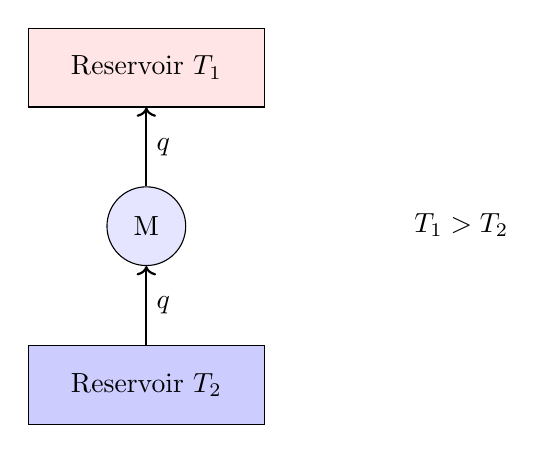
\begin{tikzpicture}
    \node (Bath1) [draw, fill=red!10, minimum width=3cm, minimum height=1cm, label=center:Reservoir $T_1$] {};
    \node (M) [draw, circle, fill=blue!10, minimum size=1cm, below=1cm of Bath1, label=center:M] {};
    \node (Bath2) [draw, fill=blue!20, minimum width=3cm, minimum height=1cm, below=1cm of M, label=center:Reservoir $T_2$] {};
    \draw [<-, thick] (Bath1.south) -- (M.north) node[midway, right] {$q$};
    \draw [<-, thick] (M.south) -- (Bath2.north) node[midway, right] {$q$};
    \node at (4, -2) {$T_1 > T_2$};
\end{tikzpicture}
\end{center}
This violates the Second Law. Over one cycle ($\Delta S_M = 0$):
$\Delta S_{tot} = \Delta S_1 + \Delta S_2 = \frac{q}{T_1} - \frac{q}{T_2} = q \left( \frac{1}{T_1} - \frac{1}{T_2} \right)$.
Since $T_1 > T_2$, $(1/T_1 - 1/T_2) < 0$. If $q>0$, then $\Delta S_{tot} < 0$. X

\textbf{Clausius Statement of the Second Law:} "It is impossible to construct a perfect refrigerator" (a device whose sole effect is to transfer heat from a colder body to a hotter body).

\textbf{A "Real" Refrigerator:} Requires work input $W$.

\begin{center}
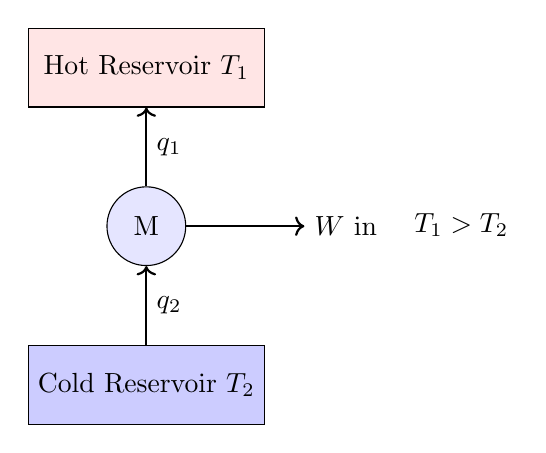
\begin{tikzpicture}
    \node (Bath1) [draw, fill=red!10, minimum width=3cm, minimum height=1cm, label=center:Hot Reservoir $T_1$] {};
    \node (M) [draw, circle, fill=blue!10, minimum size=1cm, below=1cm of Bath1, label=center:M] {};
    \node (Bath2) [draw, fill=blue!20, minimum width=3cm, minimum height=1cm, below=1cm of M, label=center:Cold Reservoir $T_2$] {};
    \draw [<-, thick] (Bath1.south) -- (M.north) node[midway, right] {$q_1$};
    \draw [->, thick] (M.east) -- ++(1.5, 0) node[right] {$W$ in}; % Work input
    \draw [<-, thick] (M.south) -- (Bath2.north) node[midway, right] {$q_2$};
    \node at (4, -2) {$T_1 > T_2$};
\end{tikzpicture}
\end{center}
First Law (over cycle): $\Delta E_M = Q_{net} - W_{net} = (q_2 - q_1) - (-W) = 0 \implies q_1 = q_2 + W$. (Heat rejected = heat absorbed + work input).
Second Law: $\Delta S_{tot} = \Delta S_1 + \Delta S_2 \ge 0 \implies \frac{q_1}{T_1} - \frac{q_2}{T_2} \ge 0$.
\[ \frac{q_2+W}{T_1} \ge \frac{q_2}{T_2} \implies \frac{W}{T_1} \ge q_2 \left( \frac{1}{T_2} - \frac{1}{T_1} \right) = q_2 \frac{T_1 - T_2}{T_1 T_2} \]
\[ W \ge q_2 \frac{T_1 - T_2}{T_2} \]
The "Coefficient of Performance" (COP) $K$ for a refrigerator is:
\[ K = \frac{q_2}{W} = \frac{\text{what we want (Heat extracted from cold)}}{\text{what we pay for (Work input)}} \]
From the Second Law inequality:
\[ K \le \frac{T_2}{T_1 - T_2} \]
The maximum COP is $K_{max} = \frac{T_2}{T_1 - T_2}$, achieved by a reversible refrigerator (e.g., reversed Carnot cycle).

\end{document}